\chapter{Description of LOBs  }
In this chapter,  we give precise mathematical descriptions of LOBs' trading and exchanging principles. 
In addition, some basic statistical properties of LOBs,  which have been proposed by past research,  are also studied and described. Those properties include size of orders,  shape of order books, time of arrival of orders,  placement of orders and so on. Study of those properties will help us get a clearer insight of how to capture the dynamics of LOBs. For example, knowing the distribution of arrival of orders will help us build more meaningful features in our prediction models. 
  
\section{Mathematical descriptions of LOBs}
In this section,  we give a relatively formal definition of LOBs and other related aspects of LOBs,  most of these definitions come from \cite{gould2013limit}. 
A LOB can be represented as a three-dimensional vector by the following definition: 
\begin{defn}\cite{gould2013limit}
An order $x=(p_x,  \omega_x, t-x)$ submitted at time $t_x$ which price $p_x$ and size $\omega_x>0$(respectively,  $\omega_x<0$) is a commitment to sell (respectively,  buy) up to $|\omega_x|$ units of the traded asset at a price no less than (respectively,  no greater than) $P_x$.
\end{defn}

For a given LOB,  the units of order size and price are defined as follows: 
\begin{defn}\cite{gould2013limit}
The lot size of a LOB is the smallest amount of the asset that can be traded within it. All orders must arrive with a size $\omega \in \{\pm k\sigma|k=1, 2, ...\}$
\end{defn}

\begin{defn}\cite{gould2013limit}
The tick size $\pi$ of a LOB is the smallest permissible price interval between different orders within it. All orders must arrive with a price that is specified to the accuracy of $\pi$
\end{defn}

For example,  if $\pi=0.01$,  then the largest permissible order price that is strictly less than \$1 is \$ 0.99,  and all orders must be submitted at a price with exactly two decimal places.
\begin{defn}\cite{gould2013limit}
The lot size $\sigma$ and tick size $\pi$ of a LOB are collectively called its resolution parameters.
\end{defn} 
\begin{defn}\cite{gould2013limit}
When a buy (respectively,  sell) order $x$ is submitted,  a LOB's trade-matching algorithm checks whether it is possible to match $x$ to some other previously submitted sell(respectively,  buy) order. If so,  the matching occurs immediately. If not,  $x$ becomes $active$
\end{defn}

Active orders in a market make up a LOB: 
\begin{defn}\cite{gould2013limit}
a LOB $\mathcal{L}(t)$ is the set of all active orders in a market at time t.
\end{defn} 

a LOB can be treated as a set of queues,  each of which contains active bid or ask orders at a specified price.
\begin{defn}\cite{gould2013limit}
The bid-side depth available at price $p$ and at time $t$ is: 
\begin{equation*}
n^b(p, t): =\sum_{\{x \in \mathcal{B}(t)|p_x=p\}}\omega_x
\end{equation*}
The ask-side depth available at price $p$ and at time $t$,  denoted $n^a(p, t)$,  is defined similarly using $\mathcal{A}(t)$
\end{defn} 

The depth available is often demonstrated as multiples of the lot size. Since $\omega_x<0$ for bid orders and $\omega_x>0$ for ask orders,  it implies that $n^b(p, t)\leq 0$ and $n^a(p, t)\geq 0$ for all prices $p$.
\begin{defn}\cite{gould2013limit}
The bid-side depth profile at time $t$ is the set of all ordered pairs($p$, $n^b(p, t)$). The ask-side depth profile at time $t$ is the set of all ordered pairs($p$, $n^a(p, t)$).
\end{defn}

\begin{defn}\cite{gould2013limit}
The mean bid-side depth available at price $p$ between times $t_1$ and $t_2$ is
\begin{equation*}
\bar{n}^b(p, t_1, t_2): =\frac{1}{t_2-t_1}\int_{t_1}^{t_2}n^b(p, t)dt
\end{equation*}

The mean ask-side depth available at price p between times $t_1$ and $t_2$,  denoted as $\bar{n}^a(p, t_1, t_2)$,  is defined similarly using the ask-side depth available.
\end{defn}

In the following,  we define the terms of \textit{bid price,  ask price,  mid price,  and bid-ask spread}
\begin{defn}\cite{gould2013limit}
The bid price at time t is the highest stated price among active buy orders at time t, 
\begin{equation*}
b(t): =\max_{x\in \mathcal{B}(t)}p_x
\end{equation*}

The ask price at time t is the lowest stated price among active sell orders at time t, 
\begin{equation*}
a(t): =\min_{x\in \mathcal{A}(t)}p_x
\end{equation*}
\end{defn}

\begin{defn}\cite{gould2013limit}
The bid-ask spread at time t is $s(t): =a(t)-b(t)$
\end{defn}

\begin{defn}\cite{gould2013limit}
The mid price at time t is $m(t): =[a(t)+b(t)]/2$
\end{defn}

More clearly,  in a LOB,  $b(t)$ is the highest price at which it is immediately possible to sell at least the lot size of the traded asset at time $t$,  and $a(t)$ is the lowest price at which it is immediately possible to buy at least the lot size of the traded asset at time $t$. Considering prices relative to $b(t)$ and $a(t)$ is helpful in some cases.

\begin{defn}\cite{gould2013limit}
For a given price p,  the bid-relative price is $\delta^b(p): =b(t)-p$ and the ask-relative price is $\delta^a(p): = p-a(t)$ 
\end{defn}

Note that here is a difference in signs between the definition of $\delta$ for the two sides: $\delta^b(p)$ defines how much smaller that $p$ is than $b(t)$ and $\delta^a(p)$ illustrates how much larger that $p$ is than $a(t)$. It is useful that we compare the properties of orders on both the bid side and the ask side of a LOB. 

\begin{defn}\cite{gould2013limit}
For a given order $x=(p_x, \omega_x , t_x)$,  the relative price of the order is : 

\begin{equation*}
\delta^x: =\left\{
\begin{aligned}
\delta^b(p_x)&\ if\ the\ order\ is\ a\ buy\ order, \\
\delta^a(p_x)&\ if\ the\ order\ is\ a\ sell\ order, \\
\end{aligned}
\right.
\end{equation*}

\end{defn}

\begin{defn}\cite{gould2013limit}
The bid-side depth available at relative price $p$ and at time $t$ is: 
\begin{equation*}
N^b(p, t)=\sum_{\{x\in \mathcal{B}(t)|\delta^x=p\}}
\end{equation*}
The ask-side depth available at relative price p and at time t,  denoted $N^a(p, t)$,  is defined similarly using $\mathcal{A}(t)$
\end{defn}

\begin{defn}\cite{gould2013limit}
The bid-side relative depth profile at time t is the set of all ordered pairs$(p, N^b(p, t)).$ The ask-side relative depth profile at time t is the set of all ordered pairs$(p, N^a(p, t))$.
\end{defn}

\begin{defn}\cite{gould2013limit}
The mean bid-side depth available at relative price $p$ between times $t_1$ and $t_2$ is: 

\begin{equation*}
\bar{N}^b(p, t_1, t_2)=\frac{1}{t_2-t_1}\int_{t_1}^{t_2}N^b(p, t)
\end{equation*}
The mean ask-side depth available at relative price $p$ between times $t_1$ and $t_2$ denoted $\bar{N}^a(p, t_1, t_2)$ is defined similarly using the ask-side relative depth available.
\end{defn}

\begin{defn}\cite{gould2013limit}
The mean bid-side relative depth profile between times $t_1$ and $t_2$ is the set of all ordered pairs$(p, \bar{N}^b(p, t_1, t_2))$. The mean ask-side relative depth profile between times $t_1$ and $t_2$ is the set of all ordered pairs $(p, \bar{N}^a(p, t_1, t_2))$ 
\end{defn}

while most traders use the relative depth profile to measure the phenomenon of LOBs,  some research has claimed that relative prices play a more important role than actual prices for defining the order arrival rates (\cite{biais1995empirical}, \cite{bouchaud2002statistical}, \cite{potters2003more}, \cite{zovko2002power}), the absolute prices at which trades occur  is basically not associated with relative depth profiles. Moreover,  relative depth profiles provide little information about the bid-ask spread and mid price. Therefore,  it is better that we combine the relative depth profiles,  bid price($b(t)$) and ask price($a(t)$) together when we consider the problem of LOBs. A completed view of the evolution of a LOB can be obtained if we consider all the information simultaneously.


\section{Data description}

In this section,   we give a detailed description of our dataset which is used for training the models. Our empirical calculations are based on a data set that describes the LOB dynamics for 5 highly liquid stocks traded on Nasdaq on one specific trading day 2012-06-21. The data
that we study originates from the LOBSTER database \cite{huang2015simulating},   which lists all  order arrivals,   limit order arrivals,   and cancellations that occur on the Nasdaq platform during 09:30 to 16:00 on each trading day. There is no trading on weekends or public holidays,   so those days are excluded in our study. According to past experience,  there might some extraordinary trading activities shortly after the opening auction or just before the close auction,   so we also exclude the data during the first 30 minutes and last 30 minutes. We use the trading platform of Nasdaq,   the tick size for each stock is $\pi = \$0.01$,   and the prices of different stocks vary a lot,   from less than 300 dollar to above 500 dollars.  We choose five stocks from information technology companies containing Apple (AAPL),   Amazon (AMZN),   Google (GOOG),  Microsoft (MSFT),   and  Intel(INTC). Table \ref{tab:statistics} lists summary statistics describing trading activity
for these 5 stocks during our sample period.
\begin{table}
	\caption{Limit order book statistics}
	\label{tab:statistics}
	\begin{center}
		\begin{tabular}{|l|c|c|c|c|c|}
			\hline
			 & AAPL & AMZN & GOOG & INTC & MSFT\\[5pt]
			 \hline
		Total number of events at the best quotes& 400391 & 269748 & 147916 & 624040 & 668765 \\[5pt]
			Percentage of  order arrivals & 1.8\% & 2.1\% & 2.5\% & 3.2\% & 1.8\% \\[5pt]
		Percentage of limit order arrivals& 51.8\% & 52.2\% & 53.4\% & 51.8\%& 50.9\%\\[5pt]
			Percentage of limit order cancellations & 44.8\% & 45.2\% & 45.2\% & 44.2\% & 47.1\%\\[5pt]		
		Mean bid-ask spread(\$)& 0.1123& 0.0122& 0.0119& 0.0131& 0.0121\\[5pt]
		Mean trade price(\$)& 45.21 & 31.32& 41.55& 24.51& 28.38\\[5pt]
		 Mean volume at the best quotes(shares)& 5129& 6739& 2088& 3508& 11419\\[5pt]
		Mean size of  orders(shares)& 621 & 738 & 359 & 571 & 861\\[5pt]
		Mean size of price - maintaining  orders & 460& 519& 270& 376& 619\\[5pt]
		\hline
		\end{tabular}
	\end{center}
\end{table}
In our data,  the non-displayable orders,   commonly called hidden orders are included. The type of the data includes:1) Submission of a new limit order data 2) Cancellation of the orders,   which will partially delete the volume of order books 3) Deletion,   which will delete all the volume of the order book 4)Execution of a visible limit order 5) Execution of a hidden limit order.  For each order,   there are 10 level of the bid and ask prices,   the bid and ask volume. Time is on a nanosecond($10^{-9}$ S) basis.
\subsection{Limit order and message order}
Table \ref{tab:message},   Table \ref{tab:type},  Table \ref{tab:direction} and Table \ref{tab:limit},   show examples of message and limit order books,  containing a message book sample,  message book event type,   message book direction and a limit order book sample. Note that execution of a sell (buy) limit order corresponds to a buyer (seller) initial trade,   i.e. Buy(sell) trade. 
\begin{table}
	\caption{Message book example,   a sample on 2012-06-21}
	\label{tab:message}
	\begin{center} 
		\begin{tabular}{|l|c|c|c|c|c|}
			\hline
			Time(sec) & Event Type & Quantity & Price & Side\\[5pt]
			 \hline
		34200.017459617& 5 &  1& 2238200& -1\\[5pt]
		34200.18960767& 1& 21& 2238100& 1 \\[5pt]
		34200.18960767&	1&	20& 2239600 & -1\\[5pt]
		34200.18960767& 1& 100& 2237500& 1 \\[5pt]
		34200.18960767& 1& 13& 2240000& -1 \\[5pt]
		34200.18960767& 1& 2& 2236500 & 1 \\[5pt]
			\hline 
		\end{tabular}
	\end{center}
\end{table}
 
 \begin{table}\renewcommand{\arraystretch}{1.2} 
 	\caption{Message book event type,   a sample on 2012-06-21}
 	\label{tab:type}
 	\begin{center} 
 		\begin{tabular}{|c|c|m{5cm}}  
 			\hline
 			Type & Description\\
 			\hline
 			1 & Placing a new limit order\\
 			
 			2 & \tabincell{c}{Cancellation, which represents deleting \\a partially volume of limit order books}\\
 			
 			3& \tabincell{c}{Deletion, which represents deleting \\all volume of limit order books}\\
 			
 			4 & Executing a visible limit order \\
 			
 			5 & Executing a hidden limit order\\
 			\hline 
 		\end{tabular}\\[3ex]
 	\end{center}
 \end{table}
  
   \begin{table}
   	\caption{Message book direction,   a sample on 2012-06-21}
   	\label{tab:direction}
   	\begin{center} 
   		\begin{tabular}{|c|c|}
   			\hline
   			Direction& Description\\
   			\hline
   			-1 & Sell limit order\\
   			1 & Buy limit order\\
   		
   			\hline 
   		\end{tabular}
   	\end{center}
   \end{table}
   
In our data,   timestamps are expressed in nano-second and prices are multiplying by 10000 to remove the decimals. Currency is in US dollars and tick size,   defined as the smallest possible gap between the ask and bid prices,   is one cent. The order quantities are constrained to positive integers . An example of our limit order book can be found in table \ref{tab:limit}. We can see the order book will be updated by a new entry in the message book. For example,   the second line in message book(table \ref{tab:message}) shows a bid order of a price 2238100 with a volume 21,   and the type of this order is submit a new order which changes the information of the order book. In the first line of table \ref{tab:limit} the best bid price is 2231800,   which is lower than the new coming bid order 2238100,   so the best bid price will be updated. We can see that in the second line of table \ref{tab:limit} the level 1 (best) bid price is changed to 2238100 with the volume 21 and the original best bid price 2231800 is transferred to the level 2 (second best) bid price.

\begin{table}
   	\caption{Limit book example of stock AMZN,   a sample on 2012-06-21}
   	\label{tab:limit}
   	\begin{center} 
   		\begin{tabular}{c c c c c c c c c}
   			\hline
   			\multicolumn{4}{c}{ Level 1} & \multicolumn{4}{c}{Level 2}&... \\
   			\hline
   			 \multicolumn{2}{c}{Ask}  & \multicolumn{2}{c}{Bid} & \multicolumn{2}{c}{Ask}  & \multicolumn{2}{c}{Bid}&... \\
   			 \hline
   			  Price & Quantity & Price& Quantity& Price& Quantity& Price & Quantity\\
   			  2239500&	100&	2231800&	100&	2239900&	100&	2230700&	200&...\\
   			  2239500& 100&	2238100&	21&	2239900&	100&	2231800&	100
   			  &...\\
   			  2239500&	100&	2238100&	21&	2239600&	20&	2231800&	100
   			  &...\\
   			  2239500&	100&	2238100&	21&	2239600&	20&	2237500&	100
   			  &...\\
   			  2239500&	100&	2238100&	21&	2239600&	20&	2237500&	100
   			  &...\\
   			  2239500&	100&	2238100&	21&	2239600&	20&	2237500&	100
   			  &...\\
   		
   			\hline 
   		\end{tabular}
   	\end{center}
\end{table} 


\subsection{Order Price,  order book volume,  order book type,   and relative depth}
Here we study some properties of order price,  order book volume,   and order book type in a given day. We can see from figure \ref{fig:aapl_price} to figure \ref{fig:msft_price},   both best ask price and best bid price are decreasing on 2012-06-21. \\
\begin{figure} [hp]
  \begin{center}
    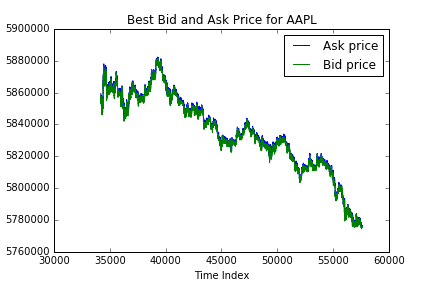
\includegraphics[width=6in,  height=5in]{figures/AAPL_price.png}
  \end{center}
\caption{Best bid and ask price of AAPL in 2012-06-21,   X-axis is the time index,   Y-axis is the prices multiply by 100,   the green line is the bid price and the blue line is the ask price} \label{fig:aapl_price}
\end{figure}
\begin{figure} [hp]
  \begin{center}
    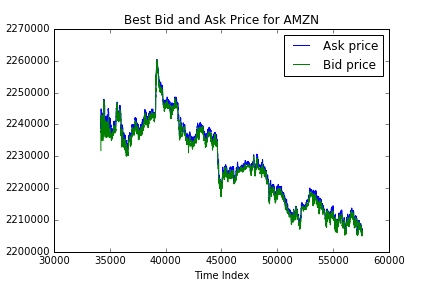
\includegraphics[width=6in,  height=5in]{figures/AMZN_price.png}
  \end{center}
\caption{Best bid and ask price of AMZN in 2012-06-21,    X-axis is the time index,   Y-axis is the prices multiply by 100,   the green line is the bid price and the blue line is the ask price} \label{fig:amzn_price}
\end{figure}

\begin{figure} [hp]
  \begin{center}
    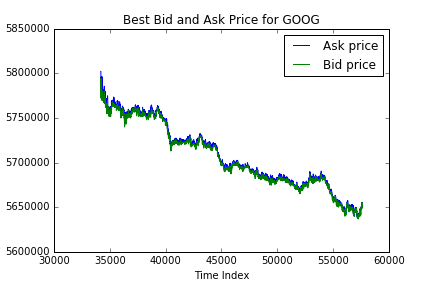
\includegraphics[width=6in,  height=5in]{figures/GOOG_price.png}
  \end{center}
\caption{Best bid and ask price of GOOG in 2012-06-21,    X-axis is the time index,   Y-axis is the prices multiply by 100,   the green line is the bid price and the blue line is the ask price} \label{fig:goog_price}
\end{figure}

\begin{figure} [hp]
  \begin{center}
    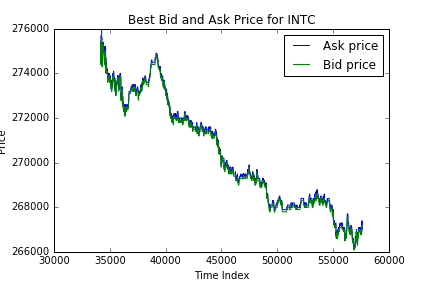
\includegraphics[width=6in,  height=5in]{figures/INTC_price.png}
  \end{center}
\caption{Best bid and ask price of INTC in 2012-06-21,    X-axis is the time index,   Y-axis is the prices multiply by 100,   the green line is the bid price and the blue line is the ask price} \label{fig:intc_price}
\end{figure}

\begin{figure} [hp]
  \begin{center}
    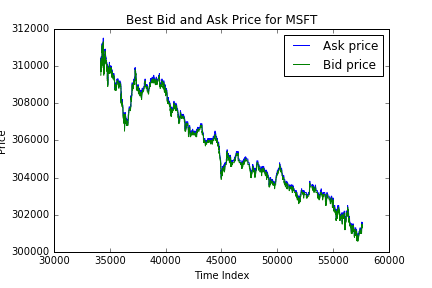
\includegraphics[width=6in,  height=5in]{figures/MSFT_price.png}
  \end{center}
\caption{Best bid and ask price of MSFT in 2012-06-21,    X-axis is the time index,   Y-axis is the prices multiply by 100,   the green line is the bid price and the blue line is the ask price} \label{fig:msft_price}
\end{figure}



\begin{figure} [hp]
  \begin{center}
    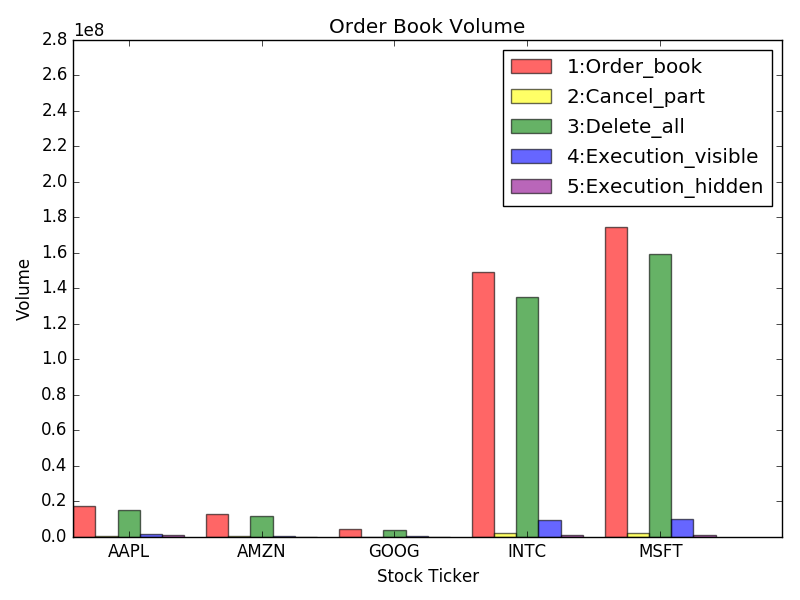
\includegraphics[width=6in,  height=5in]{figures/order_book_volume.png}
  \end{center}
\caption{Order book volume comparison for five stocks in 2012-06-21,    X-axis is the stock ticker and Y-axis is the volume of trade} \label{fig:order_book_volume}
\end{figure}

From figure \ref{fig:order_book_volume} we can see that for all the five stocks,   among all the types,   putting a new order book and canceling all the order book accounting for the vast majority of the proportion. In chapter 1,   we have mentioned that a momentum strategy will put and cancel order book in a very short time to ignite the momentum from which the executor can beneficial from the spread by other investors.

\begin{figure} [hp]
  \begin{center}
    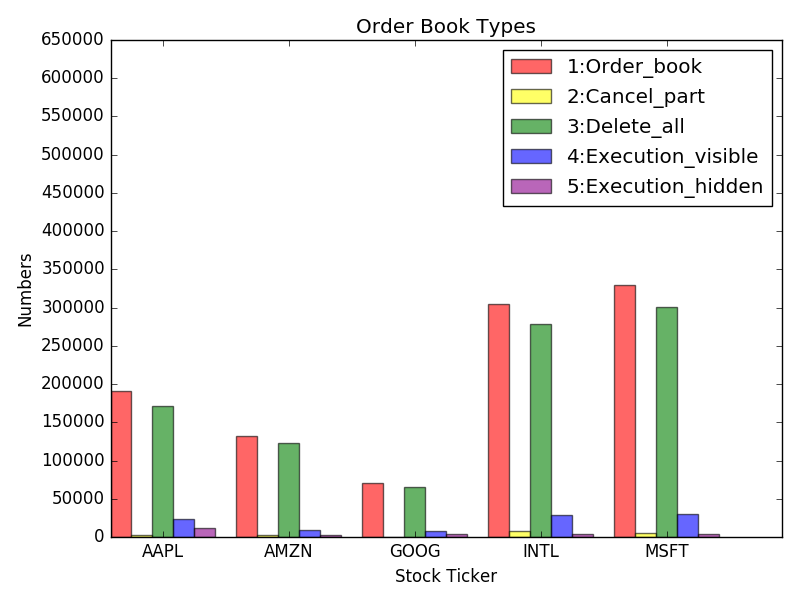
\includegraphics[width=6in,  height=5in]{figures/order_book_type.png}
  \end{center}
\caption{Order book type comparison for five stocks in 2012-06-21,  X-axis is the stock ticker and Y-axis is the number of different order book types} \label{fig:order_book_type}
\end{figure}
Figure \ref{fig:order_book_type} shows the same trend with the situation of order book volume. It is another example to show the arbitrage strategy of high-frequency trading companies. Figure \ref{fig:execution}, figure \ref{fig:volume_trade}, and figure \ref{fig:depth} show the number of trading, the volume of trading and relative depth of trading on 2012-06-21.


\begin{figure} [hp]
  \begin{center}
    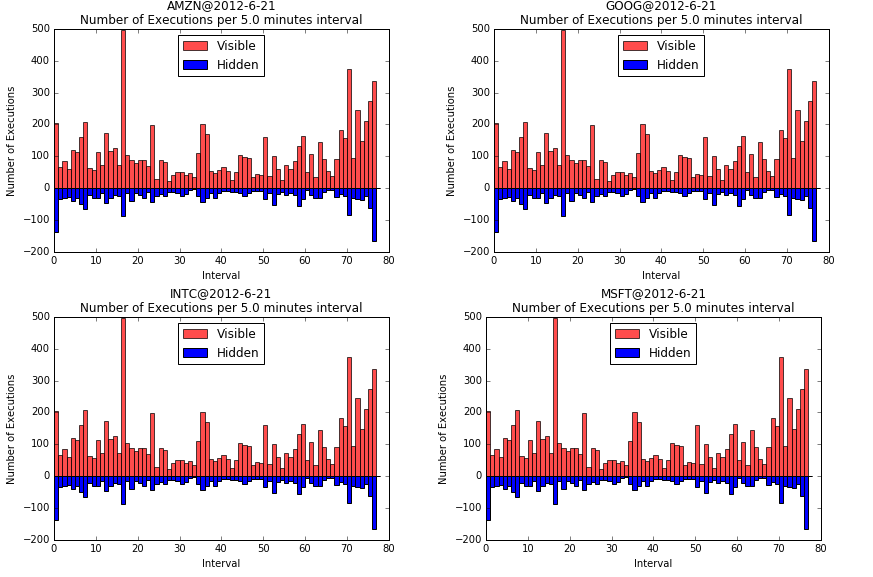
\includegraphics[width=6in,  height=5in]{figures/execution.png}
  \end{center}
\caption{Number of trading in 2012-06-21,  X-axis is the time interval and Y-axis is the number of executions. Each band in time interval represents 5 minutes.The top left panel shows the result of AMZN,   the top right panel shows the result of GOOG,  the bottom left panel shows the result of INTC,   and the bottom right panel shows the result of MSFT.   } \label{fig:execution}
\end{figure}

\begin{figure} [hp]
  \begin{center}
    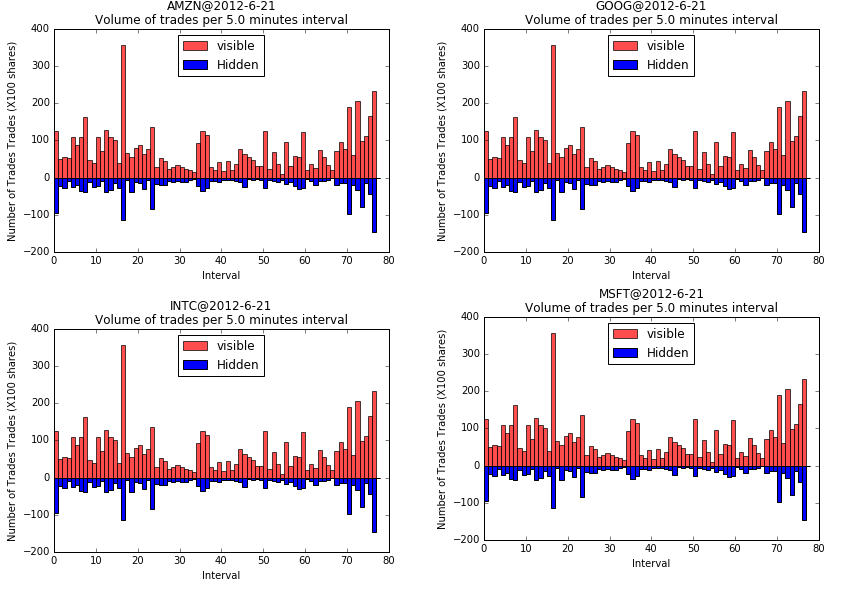
\includegraphics[width=6in,  height=5in]{figures/volume_trade.png}
  \end{center}
\caption{Volume of trading in 2012-06-21,  X-axis is the time interval and Y-axis is the number of executions. Each band in time interval represents 5 minutes.The top left panel shows the result of AMZN,   the top right panel shows the result of GOOG,  the bottom left panel shows the result of INTC,   and the bottom right panel shows the result of MSFT.  } \label{fig:volume_trade}
\end{figure}

\begin{figure} [hp]
  \begin{center}
    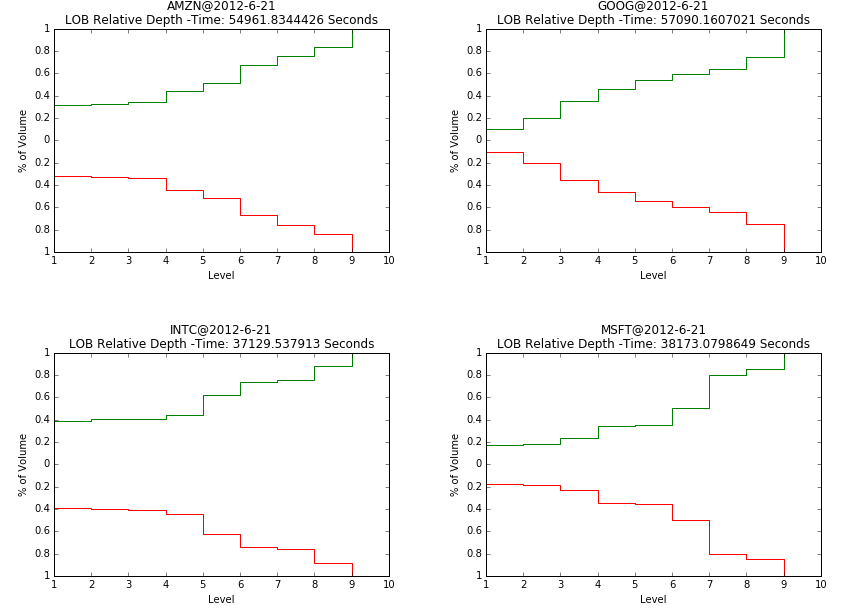
\includegraphics[width=6in,  height=5in]{figures/depth.png}
  \end{center}
\caption{Relative depth in 2012-06-21,   X-axis is the price level and Y-axis is the percentage of total volume. The top left panel shows the result of AMZN,   the top right panel shows the result of GOOG,  the bottom left panel shows the result of INTC,   and the bottom right panel shows the result of MSFT. } \label{fig:depth}
\end{figure}


\section{Properties of LOBs}
During the last two decades,  the financial market has become more and more computerized. Therefore,  it is easier for us to access extensive data on order books. To our knowledge,  \cite{biais1995empirical} is the pioneer to study the computerized data flows of Paris Bourse. After that,  a lot of related papers provide more empirical findings, statistical properties, and modeling views.(See, e.g.\cite{gopikrishnan2000statistical}, \cite{challet2001analyzing}, \cite{maslov2001price}, \cite{bouchaud2002statistical}, \cite{potters2003more}).  In this section,  we give a brief introduction of some basic empirical study results. Those fundamental statistical properties can be found through observing the real-time data. Some results of observations,  such as time of arrival of orders,  placement of orders,  size of orders,  shape of orders books and etc,  are essential for calibrating the models of order flows and capturing the dynamics of order books. 

\subsection{Time of arrivals of orders}
We compute the cumulative distribution for inter-arrival times of market orders for four stocks:  Amazon, Google,  Intel and Microsoft. The results are plotted in figure \ref{fig: arrival}.
From the figure,  it is obvious that the log-normal and exponential distribution are not good fits. The weibull distribution was suggested in \cite{ivanov2004common}.From our results,  we can see that the weibull distribution(red line in our figure) is a relatively good fit to the original data. However,  in our case,  the Gamma distribution is the best fit for each stock. 

In many past pieces of literature,  the non-Poisson arrival times models have been introduced to deal with the "irregular" financial data. For example, \cite{engle1997forecasting} and \cite{engle2000econometrics} have proposed autoregressive condition intensity models,  which are beneficial to capture the processes of orders' submission. Another research area that deals with the non-exponential arrival times relies on the branches of stochastic processes(see, e.g. \cite{clark1973subordinated};\cite{silva2007stochastic}, \cite{huth2012times}). 


\begin{figure}[hbtp]
  \begin{center}
    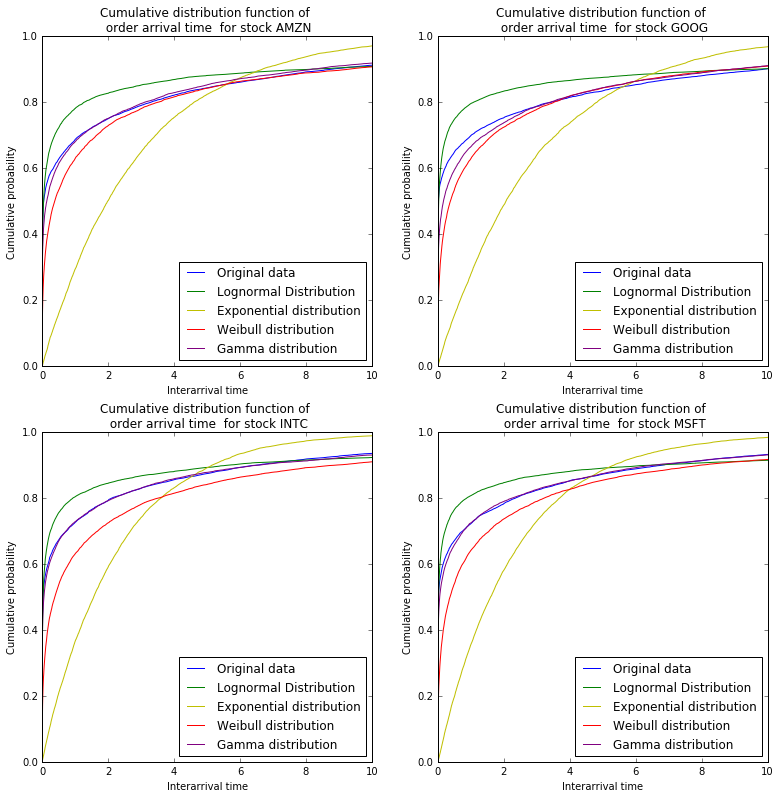
\includegraphics[width=6in, height=6in]{figures/arrival_time.png}
  \end{center}
\caption{Cumulative distribution of inter-arrival time for stock:  AMZN, GOOG, INTC and MSFT. In each panel, four distribution,  Lognormal,  Exponential Weibull and Gamma,  are compared with the original dataset. X-axis represents the inter-arrival time of market orders and Y-axis shows the cumulative probability } \label{fig: arrival}
\end{figure}


\subsection{Volume of orders}
Some past research works found that the distribution of order book sizes is difficult to measure. A widely accepted rule is power-law distribution.\cite{gopikrishnan2000statistical} and \cite{maslov2001price} find that the market orders follow a power law which decays with an exponent $1+\mu\approx2.3 \rightarrow 2.7$,  and limit orders follow a power law which decays with an exponent $1+\mu \approx 2.0$. \cite{challet2001analyzing} pay more attention to a clustering effect,  that is,  "round" size in numbers of shares of orders is often observed. Moreover,  clusters often occur around 100's and 1000's. Until now,  those research models have not reached a consensus. It makes sense that the distribution will vary greatly depending on product and market changes


\begin{figure}[hbtp]
	\begin{center}
		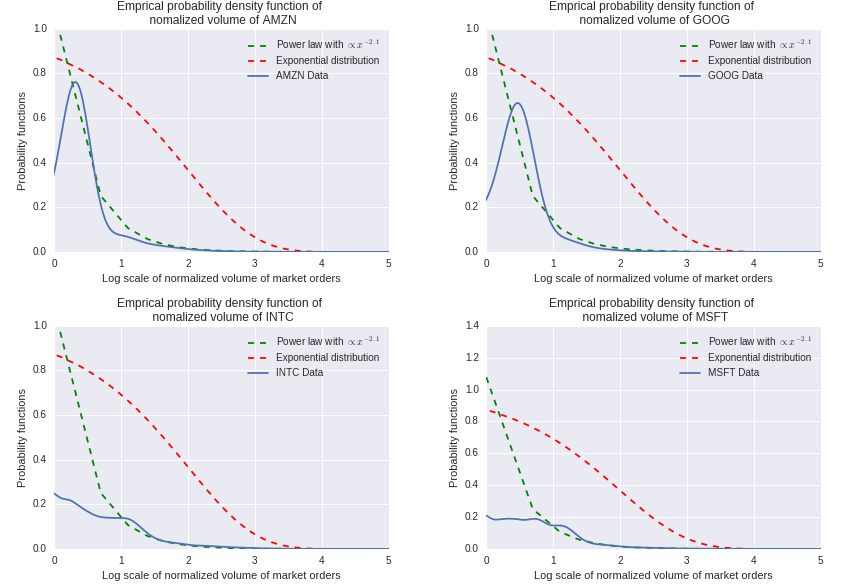
\includegraphics[width=6in, height=5in]{figures/volume.png}
	\end{center}
	\caption{Distribution of the number of orders in 5 minutes of four stocks:  AMZN, GOOG, INTC and MSFT. In each panel, power law with parameter negative 2.1 and exponential distribution  are compared with the original dataset. X-axis represents the log scale of normalized volume of market orders and Y-axis shows the probability densities of different distributions} \label{fig: volume}
\end{figure}

In figure \ref{fig: volume},  the distributions of the number of orders in 5 minutes of four stocks are plotted. We use their mean value to normalize the data. The parameter that we used in power law is negative 2.1 and the parameter that we used in exponential distribution is $1+\mu \approx 2.7$,  which we have mentioned above. We can see from the figure, in general,  the exponential distribution is better than the power function for the fitting of empirical data. Meanwhile, for AMZN and Google,  this effect is more significant.  For INTC and MSFT, there is a large deviation in the initial part.

\subsection{Placement of orders}
On the French stocks market,  \cite{bouchaud2002statistical} find that the placement of order books follows a broad power-law properties. After one year,  \cite{potters2003more} claimed the same property on the US stocks market. The parameters of the power law are relatively stable:  on the Paris Bourse,  it is $1+\mu \approx 1.6$,  on the New York Stock Exchange,  it is $1+\mu \approx 2.0$ and $1+\mu \approx 2.5$ on the London Stock Exchange. \cite{mike2008empirical} use a Student distribution with 1.3 degrees of freedom to fit the empirical distribution for LOBs. 

\begin{figure}[hbtp]
	\begin{center}
		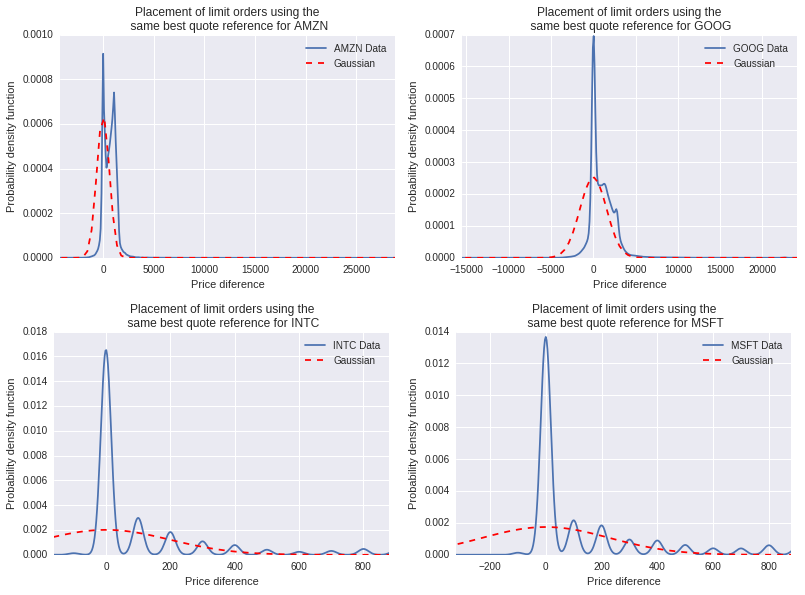
\includegraphics[width=6in, height=5in]{figures/placement.png}
	\end{center}
	\caption{Density function of placement of limit orders using the same best quote. Four stocks that we use:  AMZN, GOOG, INTC and MSFT. In each panel, Gaussian distribution is compared with the original dataset. X-axis represents the price difference between the price of arrival order and the best price before the arrival of this order. Y-axis shows the probability density function of the order book placement} \label{fig: placement}
\end{figure}

In figure \ref{fig: placement} we plot the probability distribution of placement of arriving limit orders. From this figure,  we can find that the maximum probability of placement is around 0 price difference,  which means the new order is more likely to place at the best price level. We also find heavy tails in the probability distribution,  which means that there exists some significant price difference between the new order price and the best order price.  

\subsection{Intraday seasonality} 
The financial market always changes a lot during one trading day. \cite{biais1995empirical} study the order books in Paris Bourse and observe that the numbers of order book in a given period $\Delta T$ vary a lot during the day. Figure \ref{fig: limit_vol_time} and figure \ref {fig: market_vol_time} describe the number of limit and market orders coming in a 5-minutes time intervals. From the chart,  we observe a U shape of the numbers during the whole day. The dashed line is an ordinary quadratic least square fit of the data). The U shape tells us that the market is active at the beginning and the end of the day,  and calm down around the midday. \cite{potters2003more} find that the average number of the market orders and limit orders in a $\Delta T$ period are highly correlated. In their papers,  they use millisecond data sample and we use nano-second data,  the result becomes similar,  both market order and limit order figures demonstrate a U shape. 

\begin{figure}[hbtp]
	\begin{center}
		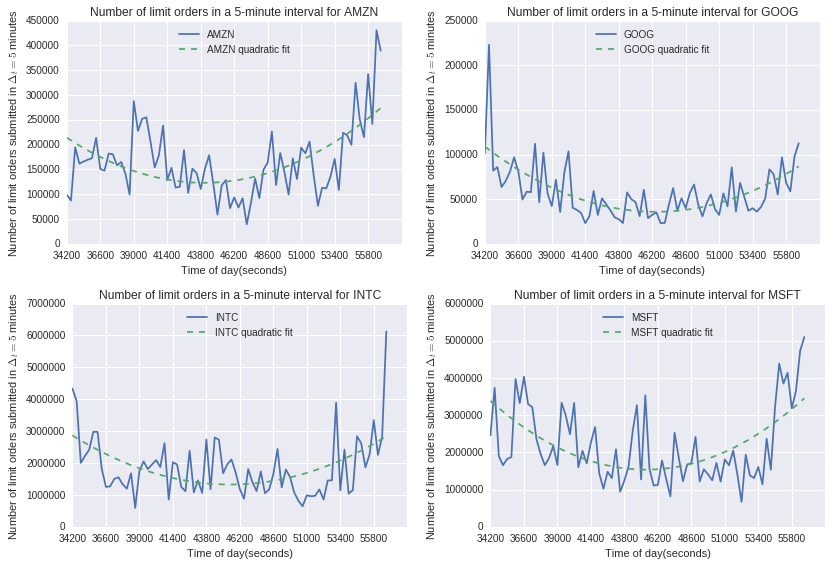
\includegraphics[width=6in, height=5in]{figures/limit_vol_time.png}
	\end{center}
	\caption{Normalized average number of limit orders in a 5-minute time interval. Four stocks that we use:  AMZN, GOOG, INTC and MSFT. In each panel, least square quadratic function is used to fit the original dataset. X-axis represents the time of day in seconds. Y-axis shows the number of limit order submitted in a 5-minute time interval} \label{fig: limit_vol_time}
\end{figure}


\begin{figure}[hbtp]
	\begin{center}
		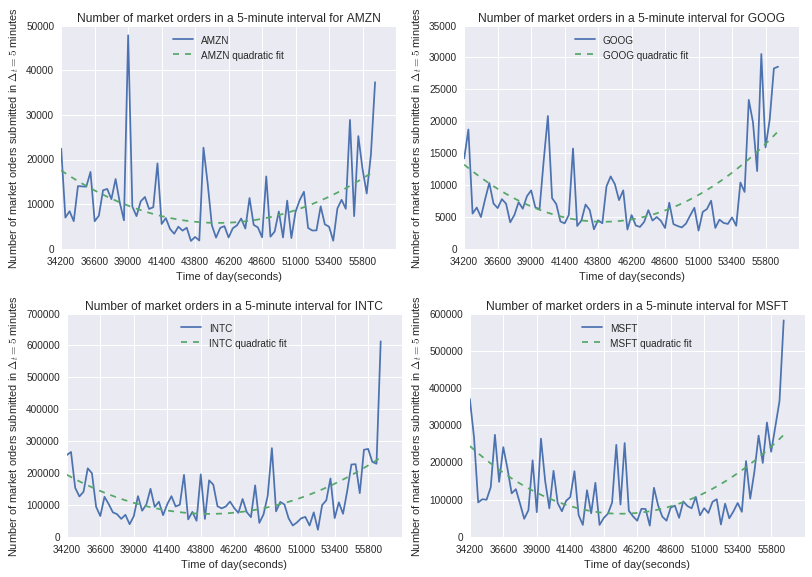
\includegraphics[width=6in, height=5in]{figures/market_vol_time.png}
	\end{center}
	\caption{Normalized average number of market orders in a 5-minute time interval. Four stocks that we use:  AMZN, GOOG, INTC and MSFT. In each panel, least square quadratic function is used to fit the original dataset. X-axis represents the time of day in seconds. Y-axis shows the number of market order submitted in a 5-minute time interval} \label{fig: market_vol_time}
\end{figure}

\subsection{Average shape of the order book}

\cite{bouchaud2002statistical} study the stocks in French capital market and find an extraordinary phenomenon that the maximum of average volume in an order book often deviates from the best price. In figure \ref {fig: level_quantity},  we plot the average number of five stocks based on a different price level. Our results show that when price level increases,  the quantity of order books tend to be large,  but not always. We can see that on the ask side of INTC,  the minimum quantity occurs at the maximum price level. This might be caused by different trading strategies and preference between the US and French financial market.   

\begin{figure}[hbtp]
	\begin{center}
		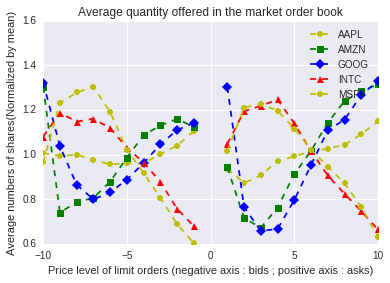
\includegraphics[width=5in, height=4in]{figures/level_quantity.png}
	\end{center}
	\caption{Average quantity of market order books. Five stocks that we use:  AAPL,  AMZN, GOOG, INTC and MSFT. X-axis represents the price level: positive axis is ask side and vice versa. Y-axis shows the average numbers of shares (normalized by mean)} \label{fig: level_quantity}
\end{figure}